\chapter{Threat Model}\label{cha:threatmodel}

\noindent
\textit{Obfuscation attacks} aim to avoid detection by strategically altering a plagiarized program, thus obscuring the relation to its original~\cite{Saglam2024b}.
As state-of-the-art detection approaches compare the structure of programs by identifying similarities between code fragments~\cite{Nichols2019}, obfuscation attacks try to alter the structural properties of the program, ideally without affecting its behavior~\cite{Novak2020, Karnalim2016, Pawelczak2018}.
The intended outcome is to disrupt the matching of fragments between programs (as seen in \autoref{tab:re-tokens}), thus leading to a reduced similarity score~\cite{DevoreMcDonald2020}.
Specifically, the goal is to prevent the detector from matching fragments above the specified match length cut-off threshold.
However, to impact the detection quality of a software plagiarism detector, the obfuscation must affect the linearized program representation of the detector, which in the case of token-based approaches is the token sequence~\cite{Saglam2024b}. Consequentially, modifications to the program code that do not affect the token sequence are inherently ineffective. For example, renaming elements like classes or members does not affect token-based approaches, as names are omitted during the tokenization~\cite{prechelt2000, Saglam2024a}.

To provide an understanding of the threat posed by automated obfuscation of plagiarism, we introduce a comprehensive threat model regarding obfuscation attacks targeting token-based software plagiarism detectors (\contribution{1}). This threat model highlights the danger of automated obfuscation attacks.
%
We focus on token-based approaches, as they are the de facto standard in practice. However, this threat model can be applied to other structure-based approaches, such as graph-based ones.

In the following, we first discuss an example of an obfuscation attack.
Second, we analyze the attack surface of token-based software plagiarism detection systems. We show that all obfuscation attacks must affect the internal program representation to disrupt the detection process.
Third, we provide a formal definition for key concepts.
Next, we categorize and relate different attack types regarding their effectiveness and applicability.
After that, we discuss the automation of obfuscation attacks via both algorithmic approaches and large language models.
Finally, we introduce the concept of \textit{intrusiveness}, which defines how much the program behavior is affected by obfuscation attempts.

\ownpublications{
\fancycite{Saglam2024b},
\fancycite{Saglam2024a},\\
and \fancycite{Saglam2024d}.
}

\section{Exemplary Obfuscation Attack}\label{sec:threatmodel-example}\label{sec:ase:RunningExample}

\noindent
We utilize the two programs depicted in \autoref{tab:running-example} as our illustrative example.
Both programs print the concatenated natural numbers from 1 to a specified maximum value. 
Notably, the variant on the right is a modified revision of the original on the left, produced via two structural changes that avoid altering the behavior of the program.
Specifically, a new variable named \texttt{debug} is inserted, and the array-style loop is replaced with a for-each loop.
Although the similarities between the two programs remain apparent for such a small example, this may not hold true when applying similar changes at a large scale.
Crucially, such alterations reduce the likelihood of detection by a plagiarism detector.

\autoref{tab:re-tokens} illustrates the internal, linearized representations of both programs. For simplicity, only the representations of the method bodies (lines 2-7) are depicted (signatures are omitted).
%These so-called token sequences contain only structural elements.
State-of-the-art plagiarism detectors linearize the programs by parsing them and extracting a subset of the parse tree nodes as \textit{tokens}~\cite{Saglam2024b}.
The resulting \textit{token sequences} consist solely of structural elements~\cite{prechelt2000}.
Details like names, types, values, and formatting are omitted, thus providing some obfuscation resilience.
Due to the modifications made to generate the variant, the token sequences of both programs are not identical.
As discussed in \autoref{sec:TPD}, all token-based software plagiarism detectors operate based on identifying common subsequences.
We can identify three matching subsequences (highlighted in grey), with each neighboring match interrupted by a single token.
Note that the differing tokens interrupt the matching. This includes a token on one side combined with the absence of one on the other and two tokens of different types on both sides.

In the example in \autoref{tab:re-tokens}, we use a cut-off threshold of two, meaning the minimum length of a match is two tokens. Matches below that length would be omitted. This value is solely chosen for illustrative purposes. In reality, the threshold would be higher. JPlag, for example, uses a default cut-off threshold of \textit{nine} tokens for Java programs and 12 tokens for C++ and Python programs. For most approaches, this threshold can also be adapted to a custom value by the user if desired.

%\todoTimur{Show that JPlag is resilient against retyping; maybe also rename a variable to show resilience against lexical changes?}

\begin{samepage}
\begin{table}[p]
	\centering
	\begin{tabular}{rlcl}
		\toprule
		\textbf{\#} & \textbf{Original}                                  &                                    & \textbf{Variant}                                \\
		\midrule
		1           & \texttt{printNumbers(int max) \{}                  &                                    & \texttt{printNumbers(int max) \{}               \\
		2           & \texttt{~~int[] n = range(0,max);}                 &                                    & \texttt{~~int[] n = range(0,max);}              \\
		3           & \texttt{~~String result = "";}                     &                                    & \texttt{~~String result = "";}                  \\
		        
		4           &                                                    & \textbf{\phantom{$\to$}  insert $\to$} & \cellcolor{add}\texttt{~~int debug = n.length;} \\
				
		5           & \cellcolor{del}\texttt{~~for(int i=0; i<max; i++)} & \textbf{$\to$ alter $\to$}   & \cellcolor{add} \texttt{~~for(int number : n)}  \\
		6           & \cellcolor{del}\texttt{~~~~result += n[i];}        & \textbf{$\to$ alter $\to$}   & \cellcolor{add} \texttt{~~~~result += number;}                  \\
		7           & \texttt{~~println(result);}                        &                                    & \texttt{~~println(result);}                     \\
		8           & \texttt{\}}                                        &                                    & \texttt{\}}                                     \\
		\bottomrule
	\end{tabular}
    \caption[Example Obfuscation: Insertion and Alteration]{Original and obfuscated programs illustrating obfuscation techniques. The original code is displayed on the left, and the obfuscated variant is on the right. The modifications include inserting a new statement in line 4, altering the loop type in line 5, and modifying a loop body statement in line 6. Removed lines are highlighted in red, and added lines are highlighted in green.}%{Original code (left) and modified variant (right) after inserting one statement and altering one. Removed lines are highlighted in red, and added lines are highlighted in green.}
	\label{tab:running-example}
\end{table}


\begin{table}[p]
	\centering
	\begin{tabular}{c
 c c cc}
		\toprule
		type & \textbf{Original Tokens} &                            & type & \textbf{Variant Tokens} \\
		\midrule
		\match 
		1  & \texttt{variable}        &                            & 1  & \texttt{variable}       \\
		\match 
		2  & \texttt{apply}           &                            & 2  & \texttt{apply}          \\
		\match 
		1  & \texttt{variable}        &                            & 1  & \texttt{variable}       \\
           &                          & \phantom{$\to$} \textbf{insert} $\to$               & \cellcolor{add}1  & \cellcolor{add}\texttt{variable}       \\
		\match 
		3  & \texttt{loop start}      &                            & 3  & \texttt{loop start}     \\
		\match 
		1  & \texttt{variable}        &                            & 1  & \texttt{variable}       \\
						         
		\cellcolor{del}4  & \cellcolor{del}\texttt{assign}          & $\to$ \textbf{remove} \phantom{$\to$} &    & \texttt{}               \\
		\match 
		4  & \texttt{assign}          &                            & 4  & \texttt{assign}         \\
		\match 
		5  & \texttt{loop end}        &                            & 5  & \texttt{loop end}       \\
		\match 
		2  & \texttt{apply}           &                            & 2  & \texttt{apply}          \\
		\bottomrule
	\end{tabular}
    \caption[Example Obfuscation Tokens: Insertion and Alteration]{Original and obfuscated token sequences corresponding to the method bodies of the programs in \autoref{tab:running-example} with three matching subsequences highlighted in gray (in detail these are $(1, 2, 1)$, $(3, 1)$, and $(4, 5, 2)$). They are interrupted by two differences in the token sequence: the insertion of a token highlighted in green, and the removal of a token highlighted in red.}
	\label{tab:re-tokens}
\end{table}

\end{samepage}
        
\section{Attack Surface Analysis}\label{sec:threatmodel-analysis}
%\todo{Examination of the attack surface of token-based plagiarism detection systems from the perspective of obfuscation attacks. Identify the entry points and vulnerabilities adversaries exploit to alter token sequences and evade detection.}

Obfuscation attacks affect the detection quality during the pairwise comparison by splitting up subsequences until they fall under the matching threshold of the detector and are thus omitted.
As token-based detectors solely use the internal representation of the programs for subsequence matching, the token-sequence, being that representation, is the only attack surface.

Consequentially, for \textit{any} obfuscation attack to be effective, it needs to affect the token sequence. Moreover, to interrupt the subsequence matching enough to reduce the calculated similarity, the attack must broadly affect the token sequence, meaning consistently over the entire sequence length. To provide an inverse example, if only the first quarter of a token sequence is altered, the matching will be disrupted only for that part. As a result, the similarity can never drop below 75 percent since that percentage of the token sequence remains matched.
Note that while the token sequence is the attack surface, it cannot be directly altered. Instead, the program code needs to be altered to lead to a different token sequence. For this reason, simple techniques like renaming have no effect on token-based approaches. While they change the program, names are not considered during the tokenization and thus do not affect the token sequence (see \autoref{sec:TPD}).

\autoref{tab:re-tokens} illustrates how the effect of the obfuscation attempts in \autoref{tab:running-example} affect the subsequence sequence matching. While only two tokens are affected, the matching is disrupted, and only three subsequences are matched. For a hypothetical cut-off threshold of four tokens, all three would be ignored, thus reducing the similarity from 100\% to 0\%. 
Note how renaming variables in the original programs would not affect the internal representation of the derived token sequences, as this type of information is not present.

As each token only encapsulates its type, meaning what kind of program element, such as control structures or variable definitions, it represents, the token sequence can be seen as a sequence of integers. \autoref{tab:re-tokens} shows this integer representation but also the type itself (e.g., apply or variable).
Based on this, there are inherently two possible atomic types of alterations: Deleting a token from the sequence and inserting a token into the sequence. We also consider changing the position of a token in the sequence as an essential alteration. However, it is technically not atomic, as it is equal to one deletion and one insertion. Note that a formal definition will follow in the subsequent section.

\begin{figure}[hb]
    \centering
    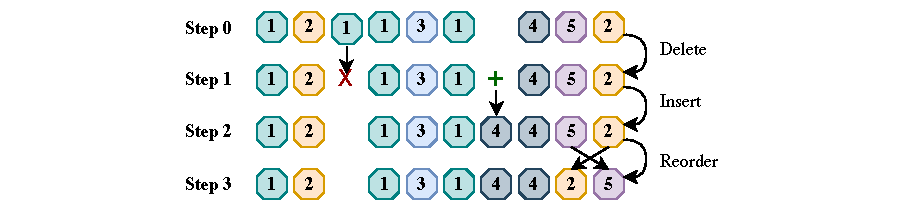
\includegraphics[width=\linewidth]{figures/atomic.pdf}
    \caption[Atomic Changes on Token Sequence Level]{Stepwise combination of three atomic modifications (token deletion, insertion, and reordering) for a token sequence. Any effective obfuscation attack must affect the token sequence.}
    \label{fig:sequence-modification}
\end{figure}

\autoref{fig:sequence-modification} illustrates these three types of alterations on example sequences.
The effects of all possible obfuscation attacks, no matter how simple or complex, can be broken down into a combination of these atomic changes.
Note that while these modifications may stem from obfuscation attacks, they can also arise when computing the difference between two unrelated programs.
Thus, the presence of certain types of changes between two token sequences alone cannot provide any indication of plagiarism.

\section{Formal Definition of Token Sequence Modification}\label{sec:threatmodel-algebra}

For plagiarism detection purposes, a linearized program can be seen as a token sequence \((a_i)_{i=1}^{l}\), where each token \(a_i\) represents a structural element of a program.
For the similarity calculation, a plagiarism detector only requires information on whether two tokens represent the same type of program element and should, therefore, be considered equivalent. 
Thus, a token sequence, in its essence, can be represented as a finite sequence of natural numbers, where each number represents a specific type of program element.

\begin{theorem}[Token Sequence]
    A token sequence \((a_i)\) is a finite sequence \((a_i)_{i=1}^{l}\) of tokens \( a_i \in \mathbb{N}\) where \(i \in \mathbb{N}\) denotes the index of a token and \(l \in \mathbb{N}\) denotes the length of the token sequence.
\end{theorem}

\begin{theorem}[Token Sequence Set]
    We define the set of all token sequences as \(\mathbf{S}\).
\end{theorem}

Plagiarism detectors compute subsequence matches to compare two token sequences and assess their similarity.
A match between two token sequences \((a_i)\) and \((b_j)\) is defined as a shared subsequence, which means it is itself a sequence that appears in both given sequences.

\begin{theorem}[Subsequence]
    Consider two token sequences \((a_i)_{i=1}^l\) and \((b_j)_{j=1}^n\). \((b_j)\) is a \textit{subsequence} of \((a_i)\), denoted by the relation
    \begin{align*}
         (b_j) \sqsubseteq (a_i)
    \end{align*}
    if 
    \begin{align*}
         \exists \, d \in \mathbb{Z} \quad \text{such that} \quad \forall j \in \{1, 2, \ldots, n\} \quad b_j = a_{j+d}.
    \end{align*}
\end{theorem}

\begin{theorem}[Subsequence Match]\label{def:subsequence-match}
    Let \((a_i)_{i=1}^l\), \((b_j)_{j=1}^n\) and \((m_k)_{k=1}^o\) be token sequences.
    Then \((m_k)\) is a subsequence match of \((a_i)\) and \((b_j)\) if
    \begin{align*}
        (m_k) \sqsubseteq (a_i) \: \land \: (m_k) \sqsubseteq (b_j).
    \end{align*}
\end{theorem}

We thus define the number of matching tokens between two token sequences as the sum of the lengths of all disjoint (non-overlapping) matching subsequences shared by the two sequences.

\begin{theorem}[Matching Tokens]\label{def:matching-tokens}
    Let \((a_i)_{i=1}^l\), \((b_j)_{j=1}^n\), and \((m_k)_{k=1}^o\) be token sequences and let \(M\) be the set of all disjoint subsequence matches for \((a_i)\) and \((b_j)\).
    We then define the number of matching tokens \(m((a_i), (b_j))\) as
    \begin{align*}
        m : \mathbf{S} \times \mathbf{S} \rightarrow \mathbb{N}
    \end{align*}
    with
    \begin{align*}
        m((a_i), (b_j)) = \sum_{(m_k) \in M}|(m_k)|
    \end{align*}
    where \(|(m_k)|\) is the length \(o\) of the token sequence \((m_k)\). Note that \(m((a_i), (b_j)) \leq l, n\).
\end{theorem} 

Since two token sequences can share multiple disjoint non-overlapping subsequences, \(m((a_i), (b_j))\) aggregates the length of all such disjoint matching subsequences. In practice, plagiarism detectors do not try to find the set of such disjoint subsequent that maximize \(m((a_i), (b_j))\); rather, they employ a greedy approach in order to find a suitable subsequence matching efficiently~\cite{Wise1993}.

The similarity of a token sequence \((a_i)\) to another sequence \((b_j)\) can be defined as the ratio of the number of matching tokens (usually based on a set of matches) to the length of the first sequence.

\begin{theorem}[Asymmetric Similarity] \label{theo:similarity}
    Let \((a_i)_{i=1}^l\), \((b_j)_{j=1}^n\) be token sequences.
    We then define similarity of \((a_i)\) to \((b_j)\) as
    \begin{align*}
    \operatorname{sim} : \mathbf{S} \times \mathbf{S} \rightarrow \mathbb{Q}
    \end{align*}
    with
    \begin{align*}
        \operatorname{sim}((a_i), (b_j)) = 
        \begin{cases}
            \frac{m((a_i), (b_j))}{l}, & \text{if } l > 0\\
            0, & \text{otherwise} .
        \end{cases}
    \end{align*}
\end{theorem}

The similarity metric \(sim\). defined in \autoref{theo:similarity} describes the proportion of tokens in sequence \((a_i)\) that are matched to tokens in sequence \((b_j)\).

It is important to note that the lengths of the token sequences \((a_i)\) and \((b_j)\) can differ.
The similarity \( {sim}_{(a_i) \rightarrow (b_j)} \) is thus not symmetric, meaning \( {sim}_{(a_i) \rightarrow (b_j)} \) is not necessarily equal to \( {sim}_{(b_j) \rightarrow (a_i)} \). However, it is used as it allows one to reason about how much of one program is matching another and vice versa.
To measure the overall similarity between two sequences, we often use symmetric metrics such as maximum similarity and symmetric similarity.

\begin{theorem}[Symmetric Similarity] \label{theo:avgsim}
    Let \((a_i)_{i=1}^l\), \((b_j)_{j=1}^n\) be token sequences.
    We then define the symmetric similarity as
    \begin{align*}
    \operatorname{symsim} : \mathbf{S} \times \mathbf{S} \rightarrow \mathbb{Q}
    \end{align*}
    with
    \begin{align*}
        \operatorname{symsim}((a_i), (b_j)) = \frac{2 \, m((a_i), (b_j))}{l+n}
    \end{align*}
\end{theorem}

\begin{theorem}[Maximum Similarity] \label{theo:maxsim}
    Let \((a_i)_{i=1}^l\), \((b_j)_{j=1}^n\) be token sequences.
    We then define the maximum similarity as
    \begin{align*}
    \operatorname{maxsim} : \mathbf{S} \times \mathbf{S} \rightarrow \mathbb{Q}
    \end{align*}
    with
    \begin{align*} 
     \operatorname{maxsim}((a_i), (b_j)) = \max(\operatorname{sim}((a_i), (b_j)),\, \operatorname{sim}((b_j), (a_i)))
\end{align*}

\end{theorem}

These metrics defined \autoref{theo:avgsim} and \autoref{theo:maxsim} provide a more comprehensive view of the similarity by considering both directions in a pairwise comparison of programs.
For simplicity, we use the term \textit{similarity} referring to the symmetric similarity throughout the remainder of this dissertation unless specified otherwise.

Finally, regarding obfuscation attacks, we previously established that they all result in a combination of fine-grained modifications of token sequences. To understand how token sequences can be modified, consider the following possible \textit{atomic} modifications:

\begin{theorem}[Token Insertion]
    Inserting a token \(t \in \mathbb{N}\) into a given token sequence \((a_i)_{i=1}^l\) at index \(k \in \mathbb{N}, k < l\) is defined as
    \begin{align*}
            \operatorname{ins} : \mathbb{N} \times \mathbf{S} \times \mathbb{N} \rightarrow \mathbf{S}
    \end{align*}
    with
    \begin{align*}
        \operatorname{ins}(t, (a_i), k) = (a_1, \dots, a_{k-1}, t, a_k, \dots, a_l)
    \end{align*}
\end{theorem}

\begin{theorem}[Token Deletion]
     Deleting a token at index \(k \in \mathbb{N},\, k < l\) in a given token sequence \((a_i)_{i=1}^l\) is defined as
    \begin{align*}
            \operatorname{del} : \mathbf{S} \times \mathbb{N} \rightarrow \mathbf{S}
    \end{align*}
    with
    \begin{align*}
        \operatorname{del}((a_i), k) = (a_1, \dots, a_{k-1}, a_{k+1}, \dots, a_l)
    \end{align*}
\end{theorem}

We also consider the following non-atomic operations as essential:

\begin{theorem}[Token Swapping]
     Swapping two tokens can be defined based on the combined insertion and deletion of two tokens,
     Given a token sequence \((a_i)_{i=1}^l\) and two indices \(k_1, k_2 \in \mathbb{N},\, k_1, k_2 \leq l \) we thus we define it as
    \begin{align*}
            \operatorname{swap} : \mathbf{S} \times \mathbb{N} \times \mathbb{N} \rightarrow \mathbf{S}
    \end{align*}
    with
    \begin{align*}
        \operatorname{swap}((a_i), k_1, k_2) = {ins}(a_{k_2}, {ins}(a_{k_1}, {del}({del}((a_i), k_1), k_2 - 1), k_2), k_1)
    \end{align*}
\end{theorem}

\begin{theorem}[Token Reordering]
    Let \((a_i)_{i=1}^l\) be a token sequence, \(\mathbf{S}_l\) be the set of all token sequences of length \(l\), and \(\mathbf{G}_l\) the set of all permutations in \(\mathbf{S}_l\)
   % Let \(\mathbf{S}_l\) be the set of all token sequences of length \(l\), and let \(\mathbf{G}_l\) be the set of all permutations
    \begin{align*}
        \sigma_l : \{1, 2, \dots, l\} \to \{1, 2, \dots, l\} \,.
    \end{align*}
    We define the reordering of tokens for sequences of length \(l\) as
    \begin{align*}
        \operatorname{reorder}_l : \mathbf{S}_l \times \mathbf{G}_l \rightarrow \mathbf{S}_l
    \end{align*}
    with
    \begin{align*}
        \operatorname{reorder}_l((a_i), \sigma) = (a_{\sigma_l(1)}, a_{\sigma_l(2)}, \dots, a_{\sigma_l(l)}) \,.
    \end{align*}
    The general reordering function is then defined as the combination of \(\operatorname{reorder}_l\) for all \(l \in \mathbb{N}\).
\end{theorem}

An obfuscation attack on a token sequence is thus defined as a set of changes to an input program that cause a series of atomic modifications to the token sequence derived from that program. The aim of such an attack is to lower the similarity of the modified token sequence to the original token sequence. Specifically, if a token sequence \((a_i)\) is a copy of another token sequence \((b_j)\), an obfuscation attack on \((a_i)\) modifies it such that the similarity falls below a threshold \(L \in \mathbb{Q}\).
Here, \(L\) is the target similarity threshold below which the similarity is deemed suspicious. Note that choosing a suitable \(L\) is up to the adversary.

\section{Categorization of Obfuscation Attacks}\label{sec:threatmodel-categorization}
The challenge for an adversary lies in finding the optimal combination of changes that maximize obfuscation\footnote{In a simplified framework, obfuscation could be seen as the opposite of similarity, e.g., along the lines of $obf_{(a_i) \rightarrow (b_j)} = 1- sim_{(a_i) \rightarrow (b_j)}$. However, not every obfuscation attempt and not every modification done as part of such an attempt is effective, which is why this relationship cannot be described so trivially.
} while minimizing the impact on the original behavior of the program.
We classify potential obfuscation attacks on a conceptual scale from verbatim copying, which is the absence of any obfuscation, to semantic clones, which are inherently hard to detect, as they have to be distinguished from unrelated, similar programs by students who did not plagiarize. Note that this scale stems from the clone type levels of \citet{Faidhi1987, Karnalim2016}. While clone detection scenarios lack the complexity of the adversarial aspects of plagiarism detection, similarities can be drawn between clone types and obfuscation types.

\autoref{fig:clone-types} illustrates this conceptual scale.
We define the following categories:
\begin{description}
    \item[Lexical Attacks] include renaming elements, changing comments, altering the code formatting, whitespace manipulation, and symbol substitution (e.g., parentheses and brackets).
    \item[Data-Based Attacks] cover type changing data types, replacing literals with equivalent but differently represented values, and adjusting the precision of numeric values.
    \item[Structural Attacks] involve fine-grained changes to the program structure, such as dead code insertion and the reordering of independent statements.
    \item[Complex Attacks] include refactoring-based attacks like changing loop types, code (de-) fragmentation, inheritance hierarchy manipulation, and modifying the control flow structure. 
    \item[Re-implementation] includes both partial re-implementation, for example, replacing a sorting algorithm with another one, as well as full implementation, which produces semantic clones.
\end{description}
Returning to our example in \autoref{tab:running-example}, statement insertion is a structural attack, while loop modification exemplifies a complex attack, albeit a simple instance.

We make no strong assumptions about the type of programming language in this categorization. While some categories or specific obfuscation attacks of a category only apply to imperative languages such as Java or C++, others apply to any given programming language.
%
Lexical Attacks apply to most languages, including functional ones.
Data-based attacks can be adapted to functional languages by manipulating data representations.
Structural Attacks, which rely on modifying the code's structure, can also be applied to functional constructs, though the way control flow is structured might differ.
Complex Attacks apply to any language, but the methods may be language-specific (e.g., recursion-heavy control flow in functional languages vs. loops in imperative ones).
Re-implementation is a concept applicable across languages.
%
Consequentially, for functional languages like Haskell, only some obfuscation attacks are valid threats. However, this means the attack space is less diverse than that of other languages. Moreover, differences in language constructs may influence the implementation of specific obfuscation techniques.
Thus, our categorization can be adapted and applied to various programming paradigms. Nevertheless, this dissertation focuses mainly on imperative languages or languages that at least support imperative constructs (e.g., Scala, F\#).
%
Consequently, no strong language-specific assumptions limit this categorization of obfuscation attacks.

Note that the categories in \autoref{fig:clone-types} are not exhaustive and may overlap in rare cases, as some obfuscation attacks may manifest in multiple categories depending on their specific implementation. Instead, they showcase different manifestations of obfuscation attacks~\cite{Novak2019, Karnalim2016}. As discussed, the attack surface for \textit{all} of these attacks remains the actual token sequence and how it affects the subsequence matching.
Moreover, as noted in the attack surface analysis, we cannot make assumptions about the presence of plagiarism or obfuscation based on the aforementioned categories alone. For example, statement insertion can be part of an obfuscation attempt, but it can also just be the difference between two unrelated solutions, where one contains these statements, such as additional debug output, while the other does not.

Token-based approaches are inherently resilient to \textit{lexical} obfuscation attacks~\cite{Joy1999}, but an adversary may nevertheless employ them to alter the appearance of the program to the human eye\footnote{To the best of our knowledge, there are no established metrics to define such a property. Also, note that this type of obfuscation is outside the scope of this dissertation, as we focus on obfuscation attacks that target software plagiarism detectors to affect their computed similarity scores.}.
Provided they employ proper tokenization, most approaches are also resilient against data-based attacks.
For instance, changing the name or value of the inserted debug statement in \autoref{tab:running-example} would not impact the derived tokens in \autoref{tab:re-tokens}.
\autoref{fig:clone-types} also illustrates the effect strength of these attack types. With rising complexity, the effect of the token sequence grows larger.
However, with rising complexity, the applicability becomes less broad. For example, dead code insertion can be applied almost everywhere in a code base, while specific refactoring attacks can only be executed where the refactoring preconditions are met~\cite{Saglam2024b}.

        \begin{figure}
            \centering
            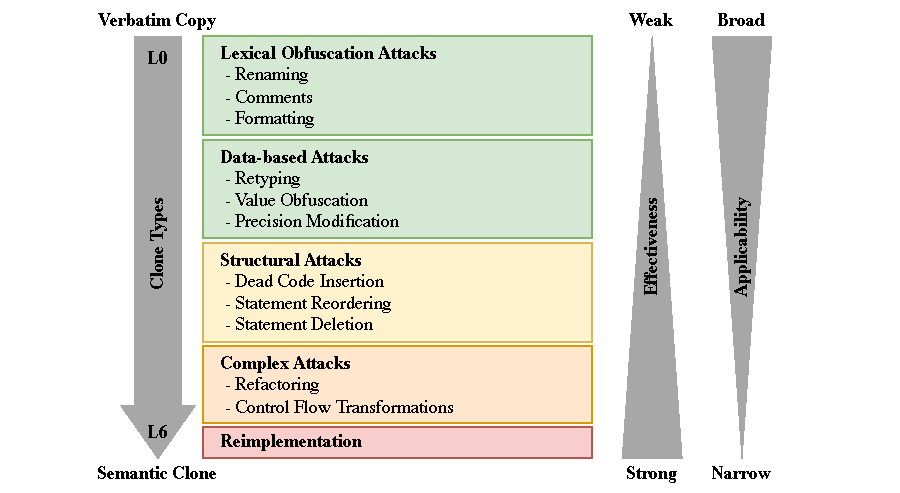
\includegraphics[width=\linewidth]{figures/threatmodel/Classification.pdf}
            \caption[Categorization of Obfuscation Attack Types]{Categorization of obfuscation attacks corresponding to the clone types by \citet{Karnalim2016, Faidhi1987}, thus illustrating the effect of the attacks on the token sequence as well as how broadly they can be applied.}
            \label{fig:clone-types}
        \end{figure}

An important limitation of our threat model concerns semantic clones. Once a certain level of re-implementation is reached, the program code may look distinct but behave identically\footnote{There is ongoing debate about what defines the behavior of a program in the context of plagiarism detection. Even fundamental questions remain contested, such as whether print statements should be considered debugging output or part of the intended behavior of a program. In practice, it depends on the educational context at hand. Methods and tools must be adapted or configured for institutions or individual courses.}. The challenge lies in accurately distinguishing these cases without erroneously flagging unrelated programs as false positives. It is worth noting that this limitation is intrinsic to plagiarism detection, whether conducted by humans or through automated tools.
Interestingly, adversaries face a similar challenge in determining the optimal extent of changes required to avoid detection while maximizing the grade or points earned and minimizing effort.
        
\section{Automation of Obfuscation Attacks}\label{sec:threatmodel-automation}
As discussed previously, automated obfuscation attacks refute the established assumption that evading detection requires more effort than completing the actual assignment~\cite{Joy1999, DevoreMcDonald2020}.
While designing such an automated attack is complicated, using it is not.

A notable example of such automated attacks is \mossad~\cite{DevoreMcDonald2020}, which repeatedly inserts (primarily dead) statements into a program to generate an obfuscated version. Statements are taken from the original program, and a pool of predefined statements called \textit{entropy}. As statements are selected randomly and inserted in random positions, this process is indeterministic and allows generating multiple plagiarized programs from one original. For each iteration, \mossad checks if the code still compiles and checks on deviating behavior by comparing the assembly code of the compiled program. This process terminates when a chosen plagiarism detector computes a similarity between the original and obfuscated version of the program that is below a targeted threshold.

\begin{theorem}[Program]\label{def:program}
For the context of this dissertation, we define a program as a function 
\begin{align*}
    P : I \rightarrow O
\end{align*}
where \(I\) is the set of all possible inputs, and \(O\) is the set of all possible outputs. Let \(\mathcal{P}\) denote the set of all programs. This simplified definition is restricted to deterministic programs and focuses on the behavior of programs.
\end{theorem}


\begin{theorem}[Threshold-Based Obfuscation]\label{def:threshold-obf} 
Let \(\mathcal{P}\) be the set of all possible programs, \(P_O \in \mathcal{P}\) be an original program, \(P_C \in \mathcal{P}\) be a verbatim copy of that program, and let \(L \in \mathbb{Q}\) denote a targeted similarity threshold.
Let \((o_i)_{i=1}^l\) denote the token sequence of \(P_O\) and \((c_j)_{j=1}^n\) denote the token sequence of \(P_C\).

We define threshold-based plagiarism as an iterative process of incrementally modifying the copy \(P_C\)
until
\begin{align*}
    \operatorname{sim}((c_i), (o_j)) < L \,.
\end{align*}
\end{theorem}

For threshold-based obfuscation (\autoref{def:threshold-obf}), any adversary usually does not know what the typical similarity of unrelated solutions for a given assignment is.
This makes estimating a suitable threshold for a threshold-based obfuscation attack an additional challenge. Thus, its values are usually chosen conservatively low. For human obfuscation, adversaries usually do not consider a specific threshold; instead, they find arbitrary criteria to determine if the obfuscation is sufficient.

\begin{theorem}[Exhaustive Obfuscation]\label{def:exhaustive-obf}
Let \(P \in \mathcal{P}\) a program in the set of all possible programs \(\mathcal{P}\) and let \(\mathcal{T} : \mathcal{P} \times \mathbb{N} \rightarrow \mathcal{P}\) be an index-based program transformation that modifies a program at a specific line index.

Given the set of line indices \(I_P \subset \mathbb{N}\) where \(\mathcal{T}\) can be applied for \(P\), we define exhaustive-based obfuscation as the process of systematically applying \(\mathcal{T}\) for any \(i \in I_P\) as follows:
\begin{align*}
    P' = \mathcal{T}(P, i) \,.
\end{align*}
\end{theorem}

For exhaustive obfuscation (\autoref{def:exhaustive-obf}), no threshold needs to be estimated by the adversary. Moreover, it increases the size of the plagiarism instances to a lesser degree than threshold-based obfuscation, as it applies a modification only once for every possible position.
However, it may be less effective than threshold-based obfuscation as it does not directly consider the similarity of a plagiarism detector.

\mossad attack is algorithmic, indeterministic, and has a threshold-based termination criterion.
Other attacks, in contrast, may be AI-based, e.g., via large language models, deterministic, or use an exhaustive termination criterion, e.g., insertion in every possible line in the code~\cite{Saglam2024a, Saglam2024b}.
This highlights the variety of potential automated attacks. Given this variety of attacks, defending against specific attack types alone is no longer sufficient. Instead, broad resilience is required.

In practice, two key questions must be considered to assess any automated obfuscation attack: First, how effective are the underlying obfuscation attack types?
Second, how easily can they be automated? 
%
More straightforward, and thus mostly fine-grained attacks, such as statement insertion, are easier to automate and can be applied more broadly across different code sections.
However, combining different attack types is more effective in obfuscating a given program.
In the past, complex attacks have been challenging to automate reliably due to their intricacy.
However, with the rise of large language models, it is relatively easy to automatically apply various obfuscation attacks to a given program~\cite{Khalil_Er_2023, Daun2023, Saglam2024a}.

However, not only the advanced effectiveness of AI-based methods makes exploiting them so viable. Just as relevant is the strongly reduced entry barrier to AI-based obfuscation. Tools like ChatGPT~\cite{ChatGPT} combine the capabilities of a large language model with the user interface of a chatbot, thus removing the need for any technical knowledge in order to use these methods.
We mention ChatGPT specifically, as it effectively kickstarted the commoditization\footnote{Only a few years ago, it was even hard for researchers to receive access to the then ground-breaking language model GPT-3. Today, there is a plethora of tools available that allow non-technical users to use language models that significantly outperform the original variant of GPT-3.} of large language models.

In the context of software plagiarism, we identify two paradigms for exploiting generative AI: \textit{Obfuscation Pre-existing Solutions} (\autoref{def:obfuscating-preexisting-solutions}) and \textit{Assignment-Driven Generation} (\autoref{def:assignment-driven-geenration}).
\begin{theorem}[Obfuscating Pre-existing Solutions]
\label{def:obfuscating-preexisting-solutions}
Let  \(\mathcal{P}_A\) be the space of solution attempts of an assignment \(A\), and let \(P_1, P_2 \in \mathcal{P}_A\) be programs representing possible solutions. We denote a program transformation relation for obfuscating pre-existing solutions as follows:
\begin{align*}
    \operatorname{obfuscate} \subseteq \mathcal{P}_A \times \mathcal{P}_A
\end{align*}
such that
\begin{align*}
    \operatorname{obfuscate}(P_1, P_2)\,.
\end{align*}
\end{theorem}

Obfuscating existing solutions involves using an existing program as input for, for example, a large language model, which is then prompted to alter the structure of the program while preserving its behavior. This process resembles human obfuscation practices and thus also involves a combination of fine-grained changes to refactor the program.
%
Note that for \autoref{def:obfuscating-preexisting-solutions}, we do not yet make any assumptions on how the obfuscation affects program behavior, as it solely defines how the plagiarism instance is created. This aspect will be discussed in the following section.

\begin{theorem}[Assignment-Driven Generation]
\label{def:assignment-driven-geenration}
Let  \(\mathcal{P}_A\) be the space of solution attempts of an assignment \(A\), let \(P \in \mathcal{P}_A\) be a program representing a possible solution, and let \(d \in \mathcal{D}_A\) be a textual description of all possible descriptions \(\mathcal{D}_A\) of \(A\).
We define a program generation relation for assignment-driven generation as follows:
\begin{align*}
    \operatorname{obfuscate} \subseteq \mathcal{D}_A \times \mathcal{P}_A
\end{align*}
such that
\begin{align*}
    \operatorname{obfuscate}(d, P)\,.
\end{align*}
\end{theorem}

Assignment-driven generation involves generating entire programs from the assignment description. However, this is technically not an obfuscation technique. Furthermore, it is currently debated whether that even qualifies as plagiarism, as there is no clear original source that is plagiarized~\cite{Novak2019}. However, in most cases, this is still considered as cheating.

Although generated solutions may exhibit higher similarity due to the semi-deterministic nature of generative AI, detecting them with low false positives is challenging. Current techniques based on generative AI exhibit \textit{some} determinism; however, they are designed to give varying output for the same input to a certain degree~\cite{Ouyang2023}.
Nevertheless, automatic obfuscation is \textit{currently}\footnote{With the rapid advancements in that field, it is essential to acknowledge that the feasibility of AI-based techniques is subject to change. Thus, these statements refer to the situation at the time of writing this dissertation.} the most effective approach for medium and larger assignments, as fully generating works only well for smaller programs~\cite{Saglam2024a, Saglam2024b}.

\section{Intrusiveness}\label{sec:intrusiveness}
An overarching consideration for the automation of attacks, regardless of whether they are AI-based or algorithmic and which termination criterion they employ, is whether the attacks alter the behavior of the target programs. Adversaries typically aim to avoid significantly altering program behavior to ensure their program still solves the given assignment. Consequently, the types of attacks are constrained, and the attack surface is limited.
\mossad, for example, avoids inserting statements that change the behavior of the program.
However, a possible scenario is accepting a limited degree of deviating behavior to achieve stronger obfuscation. Considering the threat of detection, an adversary might accept not fully solving the assignment. Defending against obfuscation attacks allowing such a deviation is even more challenging.

Therefore, obfuscation attacks can be categorized based on their level of \textit{intrusiveness}, which refers to the extent to which they alter the behavior of the target program.
The following classifications provide a framework for assessing the intrusiveness of different automated obfuscation techniques.
Note that while this categorization also applies to human obfuscation attacks, it is less relevant in those cases, as the adversary has direct control over all employed alterations.

\begin{theorem}[Functional Equivalence of Programs]\label{def:func-eq}
Let \(P_1, P_2 \in \mathcal{P}\) be programs in the set of all possible programs \(\mathcal{P}\). We say \(P_1\) and \(P_2\) are functionally equivalent denoted by the binary relation \(\equiv \, \subseteq \mathcal{P} \times \mathcal{P}\) where \(P_1 \equiv P_2\) iff \(P_1\) and \(P_2\) produce identical outputs \(o \in O\) for all inputs \(i \in I\) (see \autoref{def:program}).
\end{theorem}

Functional equivalence describes the property that two programs have the same behavior.
We base our definition of functional equivalence on \textit{contextual equivalence}, also known as \textit{observational equivalence}, as formalized by \citet{morris1969}. Contextual equivalence describes the property that two programs exhibit indistinguishable behavior under all observable \textit{contexts}. The notion of context refers to the surrounding environment in which the program executes. While this notion is a fundamental concept in programming language theory, it is generally undecidable due to the halting problem. 
Furthermore, its precise definition can vary depending on the programming language or computational model.

For plagiarism detection in educational settings, we thus use our simplified definition, focusing on observable outputs \(o \in O\) as defined by the assignment requirements, which represent a specific context.
As we refer to the context of plagiarism detection in an educational setting, what counts as \textit{output} of a given program depends on the assignments. For some assignments, any print statement is part of the behavior. An example of this is an assignment that requires students to write a command-line application. For other assignments, for example, involving a program that implements a web server, print statements may be seen as debug output and thus seen as irrelevant to the program behavior.


\begin{theorem}[Semantic-Preserving Obfuscation Attacks]\label{def:spoa}
Let  \(\mathcal{P}_A\) be the space of solution attempts of an assignment \(A\), and let \(P_1, P_2 \in \mathcal{P}_A\) be programs representing possible solutions. A program transformation relation (\autoref{def:obfuscating-preexisting-solutions})
\begin{align*}
    \operatorname{obfuscate} \subseteq \mathcal{P}_A \times \mathcal{P}_A
\end{align*}
is semantic-preserving iff
\begin{align*}
    \operatorname{obfuscate}(P_1, P_2) \quad \Rightarrow \quad P_1 \equiv P_2 \,.
\end{align*}
\end{theorem}

Semantic-preserving obfuscation Attacks are designed to maintain the original behavior of the target program. These attacks ensure that the obfuscated program performs the same tasks and produces the same outputs as the original. Plagiarism generators like \mossad and \texttt{PlagGen} explicitly check for behavioral consistency during obfuscation. Because these attacks do not alter the functionality of the program, they are preferred by adversaries who aim to avoid introducing errors that could lead to a partially correct or completely incorrect solution.

\begin{theorem}[Semantic-Agnostic Obfuscation Attacks]\label{def:saoa}
Let \(\mathcal{P}_A\) be the space of solution attempts of an assignment \(A\), and let \(P_1, P_2 \in \mathcal{P}_A\) be programs representing possible solutions. A program transformation relation (\autoref{def:obfuscating-preexisting-solutions})
\begin{align*}
    \operatorname{obfuscate} \subseteq \mathcal{P}_A \times \mathcal{P}_A
\end{align*}
is semantic-agnostic iff
\begin{align*}
    \operatorname{obfuscate}(P_1, P_2) \quad \implies \quad (P_1 \equiv P_2) \lor (P_1 \not\equiv P_2) \,.
\end{align*}
Note that the disjunction \((P_1 \equiv P_2) \lor (P_1 \not\equiv P_2)\) is always true, as the semantic-agnostic nature of the transformation implies that membership in the transformation relation does not depend on the equivalence or non-equivalence of the programs.
\end{theorem}

Semantic-agnostic obfuscation Attacks do not provide any guarantees regarding preserving the behavior of the program. While these attacks try not to alter the behavior intentionally, they also do not take steps to ensure that the behavior remains unchanged. This category includes obfuscation based on generated by large language models (LLMs) that focus on transforming the structure of the code without considering the potential impact on the behavior of the program. Although these attacks are unreliable in maintaining the correctness of the program, they can still be useful for obfuscating code while producing a mostly correct solution.

\begin{theorem}[Semantic-Deviating Obfuscation Attacks]\label{def:sdoa}
Let  \(\mathcal{P}_A\) be the space of solution attempts of an assignment \(A\), and let \(P_1, P_2 \in \mathcal{P}_A\) be programs representing possible solutions. A program transformation relation (\autoref{def:obfuscating-preexisting-solutions})
\begin{align*}
    \operatorname{obfuscate} \subseteq \mathcal{P}_A \times \mathcal{P}_A
\end{align*}
is semantic-agnostic iff
%
\begin{align*}
    \operatorname{obfuscate}(P_1, P_2) \quad \Rightarrow \quad P_1 \not\equiv P_2 \,.
\end{align*}
\end{theorem}

Semantic-deviating obfuscation attacks (or behavior-deviating attacks) accept some degree of behavioral change to achieve stronger obfuscation. These attacks might introduce modifications that alter the behavior of the program, making plagiarism harder to detect. The degree to which the behavior deviates may vary. While such techniques can provide robust obfuscation, they are generally unsuitable for situations where the correctness of the program is essential. Adversaries are thus likely to avoid behavior-altering attacks for academic assignments.

This distinction regarding intrusiveness is helpful, as it allows categorizing and reasoning about different types of obfuscation attacks. However, it is crucial to state that a difference between two programs that reflects a semantic-preserving change is not evidence for obfuscation. It is impossible to categorize and decide which modifications constitute obfuscation. Thus, we cannot simply formally define when two programs are plagiarized based on the types of differences between them. Plagiarism detection must always involve human inspection at the end, where this decision is made on a case-by-case basis (see \autoref{sec:foundations-pds} and \autoref{sec:foundations-terminology}).

In this dissertation, we primarily focus on semantic-preserving obfuscation attacks but also consider semantic-agnostic obfuscation attacks.
Semantic-preserving attacks are most feasible as they ensure the behavior of the program remains unchanged, eliminating the adversary's need for human verification of the plagiarized solution. Semantic-agnostic attacks are also practical, requiring minimal human checking since they do not deliberately alter the behavior but do not guarantee preservation.
Semantic-altering obfuscation attacks are a different challenge and thus remain out of scope.
